\documentclass[12pt]{beamer}\usepackage[]{graphicx}\usepackage[]{color}
%% maxwidth is the original width if it is less than linewidth
%% otherwise use linewidth (to make sure the graphics do not exceed the margin)
\makeatletter
\def\maxwidth{ %
  \ifdim\Gin@nat@width>\linewidth
    \linewidth
  \else
    \Gin@nat@width
  \fi
}
\makeatother

\definecolor{fgcolor}{rgb}{0.345, 0.345, 0.345}
\newcommand{\hlnum}[1]{\textcolor[rgb]{0.686,0.059,0.569}{#1}}%
\newcommand{\hlstr}[1]{\textcolor[rgb]{0.192,0.494,0.8}{#1}}%
\newcommand{\hlcom}[1]{\textcolor[rgb]{0.678,0.584,0.686}{\textit{#1}}}%
\newcommand{\hlopt}[1]{\textcolor[rgb]{0,0,0}{#1}}%
\newcommand{\hlstd}[1]{\textcolor[rgb]{0.345,0.345,0.345}{#1}}%
\newcommand{\hlkwa}[1]{\textcolor[rgb]{0.161,0.373,0.58}{\textbf{#1}}}%
\newcommand{\hlkwb}[1]{\textcolor[rgb]{0.69,0.353,0.396}{#1}}%
\newcommand{\hlkwc}[1]{\textcolor[rgb]{0.333,0.667,0.333}{#1}}%
\newcommand{\hlkwd}[1]{\textcolor[rgb]{0.737,0.353,0.396}{\textbf{#1}}}%
\let\hlipl\hlkwb

\usepackage{framed}
\makeatletter
\newenvironment{kframe}{%
 \def\at@end@of@kframe{}%
 \ifinner\ifhmode%
  \def\at@end@of@kframe{\end{minipage}}%
  \begin{minipage}{\columnwidth}%
 \fi\fi%
 \def\FrameCommand##1{\hskip\@totalleftmargin \hskip-\fboxsep
 \colorbox{shadecolor}{##1}\hskip-\fboxsep
     % There is no \\@totalrightmargin, so:
     \hskip-\linewidth \hskip-\@totalleftmargin \hskip\columnwidth}%
 \MakeFramed {\advance\hsize-\width
   \@totalleftmargin\z@ \linewidth\hsize
   \@setminipage}}%
 {\par\unskip\endMakeFramed%
 \at@end@of@kframe}
\makeatother

\definecolor{shadecolor}{rgb}{.97, .97, .97}
\definecolor{messagecolor}{rgb}{0, 0, 0}
\definecolor{warningcolor}{rgb}{1, 0, 1}
\definecolor{errorcolor}{rgb}{1, 0, 0}
\newenvironment{knitrout}{}{} % an empty environment to be redefined in TeX

\usepackage{alltt}
\usepackage{tikz}

% make it pretty
% get rid of junk
\usetheme{default}
\usefonttheme[onlymath]{serif}
\beamertemplatenavigationsymbolsempty

% define a bunch of colors
\definecolor{offwhite}{RGB}{255,250,240}
\definecolor{gray}{RGB}{155,155,155}
\definecolor{foreground}{RGB}{80,80,80}
\definecolor{background}{RGB}{255,255,255}
%\definecolor{title}{RGB}{255,199,0}
\definecolor{title}{RGB}{89,132,212}
%\definecolor{subtitle}{RGB}{89,132,212}
\definecolor{subtitle}{RGB}{255,199,0}
\definecolor{hilit}{RGB}{248,117,79}
\definecolor{vhilit}{RGB}{255,111,207}
\definecolor{lolit}{RGB}{200,200,200}
\definecolor{lit}{RGB}{255,199,0}
\definecolor{mdlit}{RGB}{89,132,212}
\definecolor{link}{RGB}{248,117,79}

% a few color macros
\newcommand{\hilit}{\color{hilit}}
\newcommand{\vhilit}{\color{vhilit}}
\newcommand{\lit}{\color{lit}}
\newcommand{\mdlit}{\color{mdlit}}
\newcommand{\lolit}{\color{lolit}}

% use those colors
\setbeamercolor{titlelike}{fg=title}
\setbeamercolor{subtitle}{fg=subtitle}
\setbeamercolor{frametitle}{fg=gray}
%\setbeamercolor{structure}{fg=subtitle}
\setbeamercolor{structure}{fg=title}
\setbeamercolor{institute}{fg=lolit}
\setbeamercolor{normal text}{fg=foreground,bg=background}
\setbeamertemplate{itemize subitem}{{\textendash}}
\setbeamerfont{itemize/enumerate subbody}{size=\small}
\setbeamerfont{itemize/enumerate subitem}{size=\small}

% center title of slides
\setbeamertemplate{blocks}[rounded]
\setbeamertemplate{frametitle}[default][center]

% page number
\setbeamerfont{page number in foot}{size=\footnotesize}
\setbeamertemplate{footline}[frame number]

% default link color
\hypersetup{colorlinks, urlcolor={link}}

% a few macros
\newcommand{\code}[1]{\texttt{#1}}
\newcommand{\hicode}[1]{{\hilit \texttt{#1}}}
\newcommand{\locode}[1]{{\lolit \texttt{#1}}}
\newcommand{\bb}[1]{\begin{block}{#1}}
\newcommand{\eb}{\end{block}}
\newcommand{\bi}{\begin{itemize}}
\newcommand{\bbi}{\vspace{4pt} \begin{itemize} \itemsep8pt}
\newcommand{\ei}{\end{itemize}}
\newcommand{\bv}{\begin{verbatim}}
\newcommand{\ev}{\end{verbatim}}
\newcommand{\ig}{\includegraphics}
\newcommand{\subt}[1]{{\footnotesize \color{subtitle} {#1}}}
\newcommand{\ttsm}{\tt \small}
\newcommand{\ttfn}{\tt \footnotesize}
\newcommand{\figh}[2]{\centerline{\includegraphics[height=#2\textheight]{#1}}}
\newcommand{\figw}[2]{\centerline{\includegraphics[width=#2\textwidth]{#1}}}



%------------------------------------------------

\title{Linear Regression (part 2)}
\subtitle{Intro 2 Statistical Learning}
\author{\href{http://www.gastonsanchez.com}{Gaston Sanchez}}
\institute{\href{https://creativecommons.org/licenses/by-sa/4.0/}{\tt \scriptsize \color{foreground} CC BY-SA 4.0}}
\date{}
\IfFileExists{upquote.sty}{\usepackage{upquote}}{}
\begin{document}



% no page number in first slide
{
  \setbeamertemplate{footline}{} 
  \frame{\titlepage} 
}

%------------------------------------------------

\begin{frame}
\begin{center}
\Huge{\hilit{Multiple Linear Regression \\ by Ordinary Least Squares}}
\end{center}
\end{frame}

%------------------------------------------------

\begin{frame}
\frametitle{Regression with various predictors}

\bbi
  \item Multiple Linear Regression
  \item $p$ predictors $\mathbf{x_1}$, $\mathbf{x_2}$, $\dots$, $\mathbf{x_p}$
  \item one response variable $\mathbf{y}$
  \item Do not confuse \textit{Multiple} with \textit{Multivariate}
  \item Multivariate Regression implies several responses \\
  (i.e. $\mathbf{y_1}$, $\dots$, $\mathbf{y_q}$)
\ei

\end{frame}

%------------------------------------------------

\begin{frame}
\frametitle{Introduction}

Suppose we observe a quantitative response $Y$ and $p$ different predictors, 
$X_1, X_2, \dots, X_p$. 

\bigskip
We assume a linear relationship of the form:
{\large
$$
Y = \beta_0 + \beta_1 X_1 + \dots + \beta_p X_p + \varepsilon
$$
}

\end{frame}

%------------------------------------------------

\begin{frame}[fragile]
\frametitle{\code{Advertising} Data}

\begin{knitrout}\scriptsize
\definecolor{shadecolor}{rgb}{0.969, 0.969, 0.969}\color{fgcolor}\begin{kframe}
\begin{alltt}
\hlcom{# file in folder data/ of github repo}
\hlstd{Advertising} \hlkwb{<-} \hlkwd{read.csv}\hlstd{(}\hlstr{"Advertising.csv"}\hlstd{,} \hlkwc{row.names} \hlstd{=} \hlnum{1}\hlstd{)}
\end{alltt}
\end{kframe}
\end{knitrout}

\begin{knitrout}\footnotesize
\definecolor{shadecolor}{rgb}{0.969, 0.969, 0.969}\color{fgcolor}\begin{kframe}
\begin{verbatim}
       TV   Radio   Newspaper   Sales
1   230.1    37.8        69.2    22.1
2    44.5    39.3        45.1    10.4
3    17.2    45.9        69.3     9.3
4   151.5    41.3        58.5    18.5
5   180.8    10.8        58.4    12.9
6     8.7    48.9        75.0     7.2
7    57.5    32.8        23.5    11.8
8   120.2    19.6        11.6    13.2
\end{verbatim}
\end{kframe}
\end{knitrout}

{\lolit (first 8 rows)}

\end{frame}

%------------------------------------------------

\begin{frame}[fragile]
\frametitle{Data set \code{Advertising}}

Response:
\bi
  \item  $Y$: \code{Sales}
\ei 

Predictors:
\bi
  \item $X_1$: \code{TV}
  \item $X_2$: \code{Radio}
  \item $X_3$: \code{Newspaper}
\ei

\bigskip
Linear model:
\begin{center}
\code{Sales} = $\beta_0$ + $\beta_1$ \code{TV} + $\beta_2$ \code{Radio} + $\beta_3$ \code{Newspaper} + $\epsilon$
\end{center}

\end{frame}

%------------------------------------------------

\begin{frame}
\frametitle{Some vector-matrix notation}

Given the actual data values, we may write the model as:
$$
y_i = \beta_0 + \beta_1 x_{i1} + \beta_2 x_{i2} + \dots + \beta_p x_{ip} + \varepsilon_i
$$
for $i = 1, \dots, n$

\pause
\bigskip
It will be more convenient to use vector-matrix notation:
{\large
$$
\mathbf{y = X \boldsymbol{\beta} + \boldsymbol{\varepsilon}}
$$
}

\end{frame}

%------------------------------------------------

\begin{frame}
\frametitle{Some vector-matrix notation}

If we consider an intercept term $\beta_0$, then we have:
$$
\underset{n\times 1}{\mathbf{y}} =  \underset{n\times (p+1)}{\mathbf{X}} \times 
\underset{(p+1)\times 1}{\boldsymbol{\beta}} + \underset{n\times 1}{\boldsymbol{\varepsilon}}
$$

which can also be represented by:
$$
\begin{bmatrix} 
y_1 \\
y_2 \\
y_3 \\
\vdots \\
y_n \\
\end{bmatrix}
=
\begin{bmatrix} 
1 & x_{11} & \cdots & x_{1p} \\
1 & x_{21} & \cdots & x_{2p} \\
1 & x_{31} & \cdots & x_{3p} \\
\vdots & \ddots & \vdots \\
1 & x_{n1} & \cdots & x_{np} \\
\end{bmatrix}
\
\begin{bmatrix} 
\beta_0 \\
\beta_1 \\ 
\vdots \\
\beta_p \\
\end{bmatrix}
+
\begin{bmatrix} 
\varepsilon_1 \\
\varepsilon_2 \\
\varepsilon_3 \\
\vdots \\
\varepsilon_n \\
\end{bmatrix}
$$

\end{frame}

%------------------------------------------------

\begin{frame}
\frametitle{Some vector-matrix notation}

If the data is \textbf{mean-centered} (i.e. $\bar{X_1} = \dots = \bar{X_p} = 0$)
$$
\underset{n\times 1}{\mathbf{y}} =  \underset{n \times p}{\mathbf{X}} \times 
\underset{p\times 1}{\boldsymbol{\beta}} + \underset{n\times 1}{\boldsymbol{\varepsilon}}
$$

which can also be represented by:
$$
\begin{bmatrix} 
y_1 \\
y_2 \\
y_3 \\
\vdots \\
y_n \\
\end{bmatrix}
=
\begin{bmatrix} 
x_{11} & \cdots & x_{1p} \\
x_{21} & \cdots & x_{2p} \\
x_{31} & \cdots & x_{3p} \\
\vdots & \ddots & \vdots \\
x_{n1} & \cdots & x_{np} \\
\end{bmatrix}
\
\begin{bmatrix} 
\beta_1 \\ 
\vdots \\
\beta_p \\
\end{bmatrix}
+
\begin{bmatrix} 
\varepsilon_1 \\
\varepsilon_2 \\
\varepsilon_3 \\
\vdots \\
\varepsilon_n \\
\end{bmatrix}
$$

\end{frame}

%------------------------------------------------

\begin{frame}
\begin{center}
\Huge{\hilit{OLS Estimation}}
\end{center}
\end{frame}

%------------------------------------------------

\begin{frame}
\frametitle{OLS Estimation}

Assuming a linear model
$$
Y = \beta_0 + \beta_1 X_1 + \dots + \beta_p X_p + \varepsilon
$$

the challenge involves finding parameter estimates denoted by 
$\hat{\beta_0}, \hat{\beta_1}, \dots, \hat{\beta_p}$ that provide the ``best''
approximation for $Y$:

$$
Y \approx \hat{\beta_0} + \hat{\beta_1} X_1 + \dots + \hat{\beta_p} X_p
$$

or more commonly

$$
\hat{Y} = \hat{\beta_0} + \hat{\beta_1} X_1 + \dots + \hat{\beta_p} X_p
$$

\end{frame}

%------------------------------------------------

\begin{frame}
\frametitle{Matrix Notation}

{\mdlit Model}
$$
\mathbf{y = X \boldsymbol{\beta} + \boldsymbol{\varepsilon}}
$$

\bigskip
{\mdlit Estimation}: fitted (or predicted) values
$$
\mathbf{\hat{y} = X \boldsymbol{\hat{\beta}} = Xb}
$$

\bigskip
{\mdlit Residuals}: observed - predicted
$$
\mathbf{e = y - \hat{y}}
$$

\end{frame}

%------------------------------------------------

\begin{frame}
\frametitle{Matrix Notation}

We want to calculate $\mathbf{b} = \boldsymbol{\hat{\beta}}$ such that $\mathbf{\hat{y}}$ is a 
good approximation of $\mathbf{y}$. 

\bigskip
The idea is to choose $\hat{\beta_0}, \hat{\beta_1}, \dots, \hat{\beta_p}$ that 
minimize the \textit{size} of the residuals:
$$
\mathbf{e = y - \hat{y} = y - Xb}
$$

What criteria should be used to minimize the \textit{size} of the residuals?

\end{frame}

%------------------------------------------------

\begin{frame}
\frametitle{Geometric illustration}
\begin{center}
\ig[width=11cm]{images/geo-least-squares1.pdf}
\end{center}
\end{frame}

%------------------------------------------------

\begin{frame}
\frametitle{Matrix Notation}

Our wish is to minimize the residuals for all $i = 1, 2, \dots, n$:
$$
e_i = y_i - \hat{y}_i
$$

Among the the possible criteria to minimize we have:
\bi
  \item $min \left \{ \sum_{i=1}^{n} e_{i}^{2} \right \} \quad$ {\lolit $L_2$-norm}
  \item $min \left \{ \sum_{i=1}^{n} |e_i| \right \} \quad$ {\lolit $L_1$-norm}
  \item $min \left \{ max(e_i) \right \} \quad$ {\lolit $L_\infty$-norm}
  \item \textit{etc}
\ei

\end{frame}

%------------------------------------------------

\begin{frame}
\frametitle{Matrix Notation}

Least Squares involves minimizing the sum of squares ($L_2$-norm): 
$$
min \left \{ \sum_{i=1}^{n} e_{i}^{2} \right \}
$$

This sum is better known as the Residual Sum of Squares ($RSS$)
$$
RSS = \sum_{i=1}^{n} e_{i}^{2}
$$

In vector-matrix notation:
$$
RSS = \mathbf{e^{\mathsf{T}} e} = \| \mathbf{e} \|^2 = \| \mathbf{y - \hat{y}} \|^2
$$

\end{frame}

%------------------------------------------------

\begin{frame}
\frametitle{Least Squares Geometry}
\begin{center}
\ig[width=11cm]{images/geo-least-squares2.pdf}
\end{center}
\end{frame}

%------------------------------------------------

\begin{frame}
\frametitle{OLS Geometric Idea}

Geometrically speaking

\bi
  \item the response lies in an $n$-dimensional space: $\mathbf{y} \in \mathbb{R}^n$
  \item the vector of parameters lies in a $p$-dimesional space: $\boldsymbol{\beta} \in \mathbb{R}^p$ 
  \item in OLS, the response is projected orthogonally onto the model space spanned by $\mathbf{X}$
  \item the fit is represented by projection $\mathbf{\hat{y} = Xb}$
  \item the difference between the fit and the data is the residual vector $\mathbf{e}$
  \item the residual vector lies in an $(n-p)$-dimensional space: $\mathbf{b} \in \mathbb{R}^{(n-p)}$
\ei

\end{frame}

%------------------------------------------------

\begin{frame}
\begin{center}
\Huge{\hilit{Least Squares Minimization}}
\end{center}
\end{frame}

%------------------------------------------------

\begin{frame}
\frametitle{OLS Minimization}

OLS Criterion:
$$
min \left \{ \sum_{i=1}^{n} e_{i}^{2} \right \} = min \left \{ \| \mathbf{e} \|^2 \right \}
$$

This means that the ``best'' $\mathbf{b}$ is the one which minimizes the $RSS$:
$$
RSS(\mathbf{b}) = \sum_{i=1}^{n} e_i^2 = \mathbf{e^{\mathsf{T}} e} = \mathbf{(y - Xb)^{\mathsf{T}} (y - Xb)}
$$

\end{frame}

%------------------------------------------------

\begin{frame}
\frametitle{OLS Minimization}

Differentiating $RSS(\mathbf{b})$ with respect to $\mathbf{b}$ yields:
$$
\frac{RSS(\mathbf{b})}{\partial \mathbf{b}} = -2 \mathbf{X^{\mathsf{T}}y} + 2 \mathbf{X^{\mathsf{T}} Xb}
$$

\pause
Equating to zero we have the so-called \textit{normal equations}:
$$
\mathbf{X^{\mathsf{T}} Xb = X^{\mathsf{T}} y}
$$

\end{frame}

%------------------------------------------------

\begin{frame}
\frametitle{OLS Minimization}

Assuming that the matrix $\mathbf{X^{\mathsf{T}} X}$ is nonsingular (invertible),
the unique ordinary least squares (OLS) estimator of $\boldsymbol{\beta}$ 
is given by: 
$$
\mathbf{b} = (\mathbf{X}^{\mathsf{T}} \mathbf{X})^{-1} \mathbf{X}^{\mathsf{T}} \mathbf{y}
$$

\pause
The fitted values are

$$
\mathbf{\hat{y}} = \mathbf{X b} = 
\mathbf{X (X^{\mathsf{T}} X)^{-1} X^{\mathsf{T}} y}
$$

\bigskip
{\mdlit What conditions are needed for $\mathbf{X^{\mathsf{T}} X}$ to be invertible?}

\end{frame}

%------------------------------------------------

\begin{frame}[fragile]
\frametitle{Example: Advertising Data}

\begin{knitrout}\footnotesize
\definecolor{shadecolor}{rgb}{0.969, 0.969, 0.969}\color{fgcolor}\begin{kframe}
\begin{alltt}
\hlcom{# number of observations}
\hlstd{n} \hlkwb{<-} \hlkwd{nrow}\hlstd{(Advertising)}

\hlcom{# model matrix}
\hlstd{X} \hlkwb{<-} \hlkwd{as.matrix}\hlstd{(Advertising[ ,}\hlkwd{c}\hlstd{(}\hlstr{'TV'}\hlstd{,} \hlstr{'Radio'}\hlstd{,} \hlstr{'Newspaper'}\hlstd{)])}
\hlstd{X} \hlkwb{<-} \hlkwd{cbind}\hlstd{(}\hlkwc{Intercept} \hlstd{=} \hlkwd{rep}\hlstd{(}\hlnum{1}\hlstd{, n), X)}

\hlcom{# response variable}
\hlstd{y} \hlkwb{<-} \hlstd{Advertising}\hlopt{$}\hlstd{Sales}
\end{alltt}
\end{kframe}
\end{knitrout}

\end{frame}

%------------------------------------------------

\begin{frame}[fragile]
\frametitle{Example: Advertising Data}

$$
\mathbf{b} = (\mathbf{X}^{\mathsf{T}} \mathbf{X})^{-1} \mathbf{X}^{\mathsf{T}} \mathbf{y}
$$

\begin{knitrout}\footnotesize
\definecolor{shadecolor}{rgb}{0.969, 0.969, 0.969}\color{fgcolor}\begin{kframe}
\begin{alltt}
\hlcom{# coefficients}
\hlstd{b} \hlkwb{<-} \hlkwd{solve}\hlstd{(}\hlkwd{t}\hlstd{(X)} \hlopt \hlstd{X)} \hlopt \hlkwd{t}\hlstd{(X)} \hlopt \hlstd{y}
\hlstd{b}
\end{alltt}
\begin{verbatim}
##                   [,1]
## Intercept  2.938889369
## TV         0.045764645
## Radio      0.188530017
## Newspaper -0.001037493
\end{verbatim}
\end{kframe}
\end{knitrout}

\end{frame}

%------------------------------------------------

\begin{frame}[fragile]
\frametitle{Example: Advertising Data}

Predicted (fitted) values:
$$
\mathbf{\hat{y}} = \mathbf{X b} = \mathbf{X (X^{\mathsf{T}} X)^{-1} X^{\mathsf{T}} y}
$$

\begin{knitrout}\footnotesize
\definecolor{shadecolor}{rgb}{0.969, 0.969, 0.969}\color{fgcolor}\begin{kframe}
\begin{alltt}
\hlcom{# fitted}
\hlstd{fitted} \hlkwb{<-} \hlstd{X} \hlopt \hlstd{b}
\end{alltt}
\end{kframe}
\end{knitrout}

\end{frame}

%------------------------------------------------

\begin{frame}[fragile]
\frametitle{Observed -vs- Predicted (fitted) values}

\begin{knitrout}\footnotesize
\definecolor{shadecolor}{rgb}{0.969, 0.969, 0.969}\color{fgcolor}

{\centering 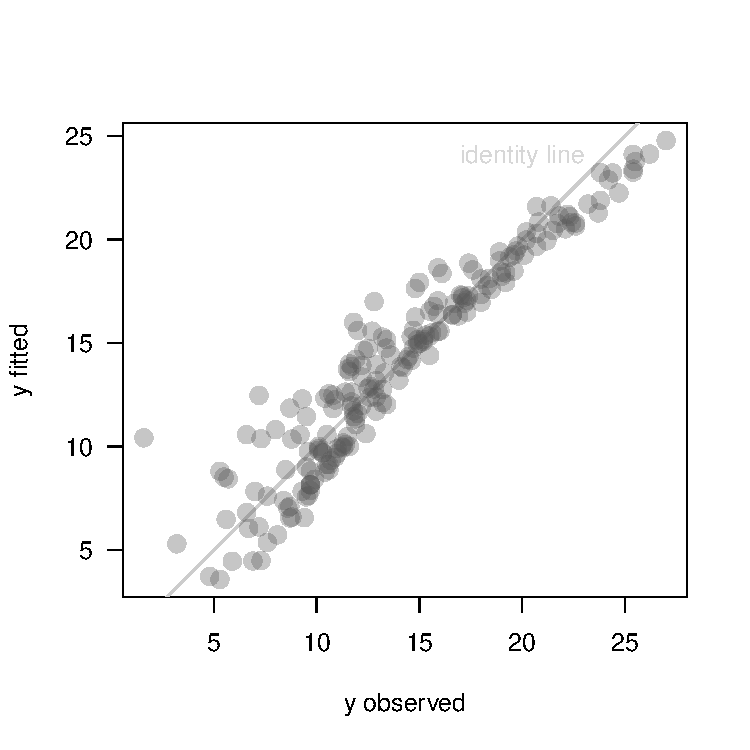
\includegraphics[width=.7\linewidth,height=.7\linewidth]{figure/obs_pred_scatter-1} 

}



\end{knitrout}

\end{frame}

%------------------------------------------------

\begin{frame}
\frametitle{OLS Minimization}

The fitted values are
$$
\mathbf{\hat{y}} = \mathbf{X b} = 
\mathbf{X (X^{\mathsf{T}} X)^{-1} X^{\mathsf{T}} y}
$$

Let $\mathbf{H} = \mathbf{X (X^{\mathsf{T}} X)^{-1} X^{\mathsf{T}}}$, then:
$$
\mathbf{\hat{y}} = \mathbf{Hy}
$$

where $\mathbf{H}$ is commonly known as the {\hilit \textbf{hat matrix}}.

\bigskip
{\mdlit What's so special about $\mathbf{H}$?}

\end{frame}

%------------------------------------------------

\begin{frame}[fragile]
\frametitle{Example: Advertising Data}

$$
\mathbf{\hat{y}} = \mathbf{H y}
$$

\begin{knitrout}\footnotesize
\definecolor{shadecolor}{rgb}{0.969, 0.969, 0.969}\color{fgcolor}\begin{kframe}
\begin{alltt}
\hlcom{# equivalent with the Hat matrix}
\hlstd{H} \hlkwb{<-} \hlstd{X} \hlopt \hlkwd{solve}\hlstd{(}\hlkwd{t}\hlstd{(X)} \hlopt \hlstd{X)} \hlopt \hlkwd{t}\hlstd{(X)}
\hlstd{y_hat} \hlkwb{<-} \hlstd{H} \hlopt \hlstd{y}
\end{alltt}
\end{kframe}
\end{knitrout}

\end{frame}

%------------------------------------------------

\begin{frame}
\frametitle{Review: projection Matrices}

Let $L \subseteq \mathbb{R}^n$ be a {\hilit linear subspace}, 
i.e. $L = span\{ \mathbf{v_1, \dots, v_k} \}$ for some 
$\mathbf{v_1, \dots, v_k} \in \mathbb{R}^n$.

\bigskip
If $V \in \mathbb{R}^{n \times k}$ contains $\mathbf{v_1, \dots, v_k}$ on its columns, then
$$
span \{ \mathbf{v_1, \dots, v_k} \} = \{ a_1 \mathbf{v_1} + \dots + a_k \mathbf{v_k} : a_1, \dots, a_k \in \mathbb{R} \} = \mathrm{col}(V)
$$

The function $F: \mathbb{R}^n \rightarrow \mathbb{R}^n$ that projects points onto $L$
is called the {\hilit projection map} onto $L$. This is actually a linear function,
$F(\mathbf{x}) = P_L \mathbf{x}$, where $P_L \in \mathbb{R}^{n \times n}$ is the 
{\hilit projection matrix} onto $L$.

\end{frame}

%------------------------------------------------

\begin{frame}
\frametitle{Review: projection Matrices}

A projection matrix $P_L \in \mathbb{R}^{n \times n}$
\bi
  \item is a linear transformation
  \item is symmetric: $P_L = P^{\mathsf{T}}_{L}$
  \item is idempotent: $P_{L}^{2} = P_L$
  \item Furthermore:
  \bi
    \item $P_L \mathbf{x} = \mathbf{x}$ for all $\mathbf{x} \in L$
    \item $P_L \mathbf{x} = \mathbf{0}$ for all $\mathbf{x} \perp L$
  \ei
\ei

\end{frame}

%------------------------------------------------

\begin{frame}
\frametitle{The Hat matrix}

\bi
  \item $\mathbf{H}$ is a linear transformation
  \item $\mathbf{H}$ is symmetric: $\mathbf{H = H^{\mathsf{T}}}$
  \item $\mathbf{H}$ is idempotent: $\mathbf{H = H^2}$
  \item The hat matrix is an \textbf{orthogonal projector} or \textit{projection matrix}
  \item $\mathbf{Q = I - H}$ is the orthogonal complement or \\
  ``counterpart'' of $\mathbf{H}$
\ei

\end{frame}

%------------------------------------------------

\begin{frame}
\frametitle{Least Squares Geometry}
\begin{center}
\ig[width=11cm]{images/geo-least-squares-full.pdf}
\end{center}
\end{frame}

%------------------------------------------------

\begin{frame}
\frametitle{About the Hat matrix $\mathbf{H}$}

The theoretical model $\mathbf{y = X \boldsymbol{\beta}} + \boldsymbol{\varepsilon}$
defines a decomposition of $\mathbf{y}$ in two unknown terms:
\bbi
  \item $X \boldsymbol{\beta} \in \mathbb{R}_X$
  \item $\boldsymbol{\varepsilon} \in \mathbb{R}^n$
\ei

\end{frame}

%------------------------------------------------

\begin{frame}
\frametitle{Least Squares Geometry}
\begin{center}
\ig[width=11cm]{images/geo-least-squares-full-labeled.pdf}
\end{center}
\end{frame}

%------------------------------------------------

\begin{frame}
\frametitle{About the Hat matrix $\mathbf{H}$}

The theoretical model $\mathbf{y = X \boldsymbol{\beta}} + \boldsymbol{\varepsilon}$
defines a decomposition of $\mathbf{y}$ in two unknown terms:
\bi
  \item $X \boldsymbol{\beta} \in \mathbb{R}_X$
  \item $\boldsymbol{\varepsilon} \in \mathbb{R}^n$
\ei

\pause
The OLS method proposes a solution $\mathbf{y = Xb + e}$ that minimizes the 
``length'' of the residual vector $\mathbf{e}$ by orthogonally projecting
$\mathbf{y}$ as $\mathbf{Xb}$ in the spanned space of $\mathbf{X}$, and by 
projecting $\boldsymbol{\varepsilon}$ as $\mathbf{e}$ in the subspace
to $\mathbb{R}_X$.

\end{frame}

%------------------------------------------------

\begin{frame}
\frametitle{Residuals and Theoretical Errors}

The \textit{residuals} $\mathbf{e = y - \hat{y}}$ are the OLS estimates of the unobservable erros $\boldsymbol{\varepsilon}$.

\bigskip
The residual vector can also be written as:
$$
\mathbf{e = y - Xb = (I - H) \boldsymbol{\varepsilon} = Q \boldsymbol{\varepsilon}}
$$

\end{frame}

%------------------------------------------------

\begin{frame}[fragile]
\frametitle{Example: Advertising Data}

$$
\mathbf{e = y - Xb = (I - H) \boldsymbol{\varepsilon} = Q \boldsymbol{\varepsilon}}
$$

\begin{knitrout}\footnotesize
\definecolor{shadecolor}{rgb}{0.969, 0.969, 0.969}\color{fgcolor}\begin{kframe}
\begin{alltt}
\hlcom{# residuals}
\hlstd{residuals} \hlkwb{<-} \hlstd{y} \hlopt{-} \hlstd{y_hat}
\end{alltt}
\end{kframe}
\end{knitrout}

\end{frame}

%------------------------------------------------

\begin{frame}
\begin{center}
\Huge{\hilit{Computation}}
\end{center}
\end{frame}

%------------------------------------------------

\begin{frame}[fragile]
\frametitle{OLS Solution}

The vector of OLS estimates $\mathbf{b}$ is given by 
$\mathbf{(X^\mathsf{T} X)^{-1} X^\mathsf{T} y}$

\bigskip

In R, you may calculate $\mathbf{b}$ with something like this:
\begin{knitrout}\footnotesize
\definecolor{shadecolor}{rgb}{0.969, 0.969, 0.969}\color{fgcolor}\begin{kframe}
\begin{alltt}
\hlcom{# beta coefficients}
\hlstd{XtXi} \hlkwb{<-} \hlkwd{solve}\hlstd{(}\hlkwd{t}\hlstd{(X)} \hlopt \hlstd{X)}
\hlstd{b} \hlkwb{<-} \hlstd{XtXi} \hlopt \hlkwd{t}\hlstd{(X)} \hlopt \hlstd{y}
\end{alltt}
\end{kframe}
\end{knitrout}

\end{frame}

%------------------------------------------------

\begin{frame}
\frametitle{OLS Solution}

Although this works, computationally it is not the best way to compute 
$\mathbf{b}$.

\bigskip
Most computer programs don't compute $\mathbf{(X^\mathsf{T} X)^{-1}}$ directly.
Instead, they typically use the QR decomposition.

\end{frame}

%------------------------------------------------

\begin{frame}
\frametitle{QR Decomposition}

Any matrix $\mathbf{X}$ can be written as:

$$
\mathbf{X = QR}
$$

where:

\bi
  \item $\mathbf{Q}$ is an $n \times p$ orthogonal matrix: \\
$\mathbf{Q^\mathsf{T} Q} = \mathbf{Q Q^\mathsf{T}} = \mathbf{I}$
  \item $\mathbf{R}$ is a $p \times p$ upper triangular matrix
\ei

\end{frame}

%------------------------------------------------

\begin{frame}
\frametitle{OLS solution via QR Decomposition}

\begin{align*}
\mathbf{b} &= \mathbf{(X^\mathsf{T} X)^{-1} X^\mathsf{T} y} \\
 &= \left ( \mathbf{(QR)^\mathsf{T} QR} \right )^{-1} (\mathbf{QR})^\mathsf{T} \mathbf{y} \\
 &= \mathbf{(R^\mathsf{T} Q^\mathsf{T} Q R)^{-1} R^\mathsf{T} Q^\mathsf{T} y} \\
 &= \mathbf{(R^\mathsf{T} R)^{-1} R^\mathsf{T} Q^\mathsf{T} y} \\
 &= \mathbf{R^{-1} (R^{-\mathsf{T}} R^\mathsf{T}) Q^\mathsf{T} y} \\
 &= \mathbf{R^{-1} Q^\mathsf{T} y} 
\end{align*}

\end{frame}

%------------------------------------------------

\begin{frame}
\frametitle{OLS solution via QR Decomposition}

\begin{align*}
\mathbf{b} &= \mathbf{(X^\mathsf{T} X)^{-1} X^\mathsf{T} y} \\
 &= \mathbf{R^{-1} Q^\mathsf{T} y} 
\end{align*}

\bi
  \item we don't really want to invert $\mathbf{R}$
  \item we just want to recognize that we have a new system:
  $$
  \mathbf{R b} = \mathbf{Q^\mathsf{T} y}
  $$
  \item In practice you apply some backsubstitution routine to solve such system 
  {\lolit (you'll do that in the lab)}
\ei

\end{frame}

%------------------------------------------------

\begin{frame}
\begin{center}
\Huge{\hilit{Assessing the \\ Quality of the Fit}}
\end{center}
\end{frame}

%------------------------------------------------

\begin{frame}
\frametitle{Assessing the quality of the fit}
\begin{center}
\ig[width=11cm]{images/geo-least-squares2.pdf}
\end{center}
\end{frame}

%------------------------------------------------

\begin{frame}

Assuming that the data is mean-centered, then the lengths of the vectors in 
$\mathbb{R}^n$ can be interpreted in term of variances.

\bigskip
The Pythagoras theorem applied to the square triangle can be written as:
$$
\mathbf{y^{\mathsf{T}} y = e^{\mathsf{T}} e + b^{\mathsf{T}} X^{\mathsf{T}} X b}
$$

\bigskip
equivalently:
$$
\| \mathbf{y} \|^2 = \| \mathbf{Xb} \|^2 + \| \mathbf{e} \|^2
$$

\end{frame}

%------------------------------------------------

\begin{frame}
\frametitle{Assessing the quality of the fit}
\begin{center}
\ig[width=9cm]{images/geo-least-squares2.pdf}
\end{center}

$$
\| \mathbf{y} \|^2 = \| \mathbf{Xb} \|^2 + \| \mathbf{e} \|^2
$$

\end{frame}

%------------------------------------------------

\begin{frame}

The Pythagoras theorem:
$$
\mathbf{y^{\mathsf{T}} y = e^{\mathsf{T}} e + b^{\mathsf{T}} X^{\mathsf{T}} X b}
$$

can be reexpressed as:
$$
\sum (y_i)^2 = \sum (y_i - \hat{y}_i)^2 + \sum (\hat{y}_i)^2
$$


Dividing by $n$, we put things in terms of variances:
$$
\frac{1}{n} \sum (y_i)^2 = \frac{1}{n} \sum (y_i - \hat{y}_i)^2 + \frac{1}{n} \sum (\hat{y}_i)^2
$$

\end{frame}

%------------------------------------------------

\begin{frame}
\frametitle{Variance Decomposition}

{\large
$$
\underbrace{ \frac{1}{n} \sum (y_i)^2}_{\text{total variance}} = 
\underbrace{ \frac{1}{n} \sum (y_i - \hat{y}_i)^2}_{\text{residual variance}} + 
\underbrace{ \frac{1}{n} \sum (\hat{y}_i)^2}_{\text{explained variance}}
$$
}

\end{frame}

%------------------------------------------------

\begin{frame}
\frametitle{Multiple Correlation Coefficient}

We define the {\hilit coefficient of multiple correlation} as
$$
R^2 = cor^2(\mathbf{y, \hat{y}}) = cor^2(\mathbf{y, Xb})
$$

$R^2$ can be expressed in various forms:
$$
R^2 = \frac{cov^2(\mathbf{y, \hat{y}})}{var(\mathbf{y}) var(\mathbf{\hat{y}})} =
\frac{var({\mathbf{\hat{y}})}}{var(\mathbf{y})} = 
\frac{\text{explained variance}}{\text{total variance}}
$$

\end{frame}

%------------------------------------------------

\begin{frame}[fragile]
\frametitle{Multiple Correlation}

$$
R^2 = cor^2(\mathbf{y, \hat{y}}) = cor^2(\mathbf{y, Xb})
$$

\begin{knitrout}\footnotesize
\definecolor{shadecolor}{rgb}{0.969, 0.969, 0.969}\color{fgcolor}\begin{kframe}
\begin{alltt}
\hlcom{# coefficient of mulitple correlation}
\hlstd{R2} \hlkwb{<-} \hlkwd{cor}\hlstd{(y, y_hat)}
\hlstd{R2}
\end{alltt}
\begin{verbatim}
##          [,1]
## [1,] 0.947212
\end{verbatim}
\end{kframe}
\end{knitrout}

$R^2$ is the proportion of the variability in $\mathbf{y}$ explained
by the model

\end{frame}

%------------------------------------------------

\begin{frame}
\frametitle{Multiple Correlation Coefficient}

$R^2$ describes the fraction of the total variance of $\mathbf{y}$ that is 
explained by $\mathbf{\hat{y}}$

\bigskip
By minimzing $\sum_{i=1}^{n} e_{i}^{2}$, we actually maximize $R^2$. \\
{\mdlit What does this mean?}

\pause
\bigskip
In other words, the OLS fit provides a linear combination of the predictors
that has maximum correlation with the response variable $\mathbf{y}$.

\end{frame}

%------------------------------------------------

\begin{frame}
\frametitle{Assessing the quality of the fit}
\begin{center}
\ig[width=9cm]{images/geo-least-squares2.pdf}
\end{center}

$$
\| \mathbf{y} \|^2 = \| \mathbf{Xb} \|^2 + \| \mathbf{e} \|^2
$$

\end{frame}

%------------------------------------------------

\begin{frame}[fragile]
\frametitle{Assessing the quality of the fit}

$$
\| \mathbf{y} \|^2 = \| \mathbf{\hat{y}} \|^2 + \| \mathbf{e} \|^2
$$

$$
\sum_{i=1}^{n} (y_i - \bar{y})^2 = \sum_{i=1}^{n} (\hat{y_i} - \bar{y})^2 + \sum_{i=1}^{n} e_i^2
$$

$$
R^2 = \frac{\| \mathbf{\hat{y}} \|^2}{\| \mathbf{y} \|^2} = cos^2 (\mathbf{y}, \mathbf{\hat{y}})
$$

\end{frame}

%------------------------------------------------

\begin{frame}
\frametitle{Assessing the quality of the fit}
\begin{center}
\ig[width=10cm]{images/geo-R2.pdf}
\end{center}
\end{frame}

%------------------------------------------------

\begin{frame}
\frametitle{About $R^2$}

\bbi
  \item $R^2$ is one way to measure the quality of the fit.
  \item It doesn't tell you how accurate the coefficients are.
  \item It is a measure of \textit{resubstitution error}. \\
  (not of generalization error)
  \item It depends on the number of predictors $p$.
  \item It is interesting from the theoretical-geometric point of view.
  \item But in practice it does not say much about the predictive
  performance of a model.
\ei

\end{frame}

%------------------------------------------------

\begin{frame}
\frametitle{Some Comments}

\bbi
  \item There is nothing in the Least Squares method that requires statistical inference:
formal tests of null hypotheses or confidence intervals.
  \item In its simplest form, regression analysis can be performed without statistical inference.
  \item We will study the inferential framework in the next slides.
\ei

\end{frame}

%------------------------------------------------

\begin{frame}
\frametitle{Bibliography}

{\footnotesize
\bi
  \item \textbf{Statistical Regression and Classification} by Norman Matloff (2017). CRC Press.
  \item \textbf{Linear Models with R} by Julian Faraway (2015). CRC Press.
  \item \textbf{Modern Regression Methods} by Thomas Ryan (2009). Wiley.
  \item \textbf{A Modern Approach to Regression with R} by Simon Sheather (2009). Springer.
  \item \textbf{Modern Multivariate Statistical Techniques} by Julian Izenman (2008). Springer.
  \item \textbf{Data Mining and Statistics for Decision Making} by Stephane Tuffery (2011).
  \textit{Chapter 11: Classification and prediction methods}. Wiley.
\ei
}

\end{frame}

%------------------------------------------------

\begin{frame}
\frametitle{French Literature}

{\footnotesize
\bi
  \item \textbf{Probabilites, analyse des donnees et statistique} by Gilbert Saporta (2011).
  \textit{Chapter 17: La regression multiple et le modele lineaire general}. 
  Editions Technip, Paris.
  \item \textbf{Statistique: Methodes pour decrire, expliquer et prevoir} 
  by Michel Tenenhaus (2008). \textit{Chapter 5: La Regression Multiple}. Dunod, Paris.
  \item \textbf{Regression avec R} by Cornillon and Matzner-Lober (2011). Springer.
  \item \textbf{Statistique Exploratoire Multidimensionnelle} by Lebart et al (2004).
  \textit{Chapter 3, section 3.2: Regression multiple, modele lineaire}. Dunod, Paris.
  \item \textbf{Traitement des donnees statistiques} by Lebart et al. (1982). 
  \textit{Unit 3: Modele Lineaire}. Dunod, Paris.
\ei
}

\end{frame}

%------------------------------------------------

\end{document}
